\section{Further Evidence on the Household}\label{app:other}

This appendix reports evidence that bears on the model's assumptions but not on the headline fact.

\subsection{Intergenerational mobility by race in the PSID}\label{sec:measurement}

Following \citet{lee2009trends} and \citet{palomino2018one}, each year a son or daughter is observed at 25--65, his or
her log family income is regressed on the log of parental family income averaged over the child's ages 13--19, with
quartics in the parent's age and in the child's age minus 40 and their interactions with parental income, so that the
coefficient is the IGE at age 40. The IGE of family income is 0.27 for Black and 0.47 for White sons, and 0.29 and 0.45
for daughters; on the PSID's main sample, the pooled estimate for sons in 1980--2010 is 0.48, close to the 0.47 of
\citet{palomino2018one}. Following \citet{chetty2020race}, the rank--rank slopes are similar for the two races (0.37 for
Black and 0.39 for White children), but at the 25th percentile of parental income Black children reach a household
income rank of 28.7 and White children 41.6, a gap of 12.9 percentiles, against 12.6 in \citet{chetty2020race}. The
reliability ratio of a single year of family income is about 0.57 for both races \citep{bolt2024intergenerational}.
Code: \texttt{IGE/6.IGEMain.py}, \texttt{IGE/5.CheckPMR.py}, \texttt{IGE/7.RankMobility.py}, \texttt{IGE/4.Estimates.py}.

\subsection{Husbands' industry shocks around a birth}\label{sec:birthshocks}

If mothers insured their husbands' risk in anticipation, their work around a birth would respond to shocks to the
husband's industry. I relate married mothers' work after a birth to national employment growth of men in the husband's
sector (leaving out his state) relative to its trend, with state, year and sector fixed effects. The shock moves the
husband's own hours: one percentage point more growth in his sector raises his hours in the birth year by 5.6 (s.e.\
2.6; wild-bootstrap $p=0.040$ with 16 sector clusters). His wife's work does not respond: the effect on her employment in
the year after the birth is $-0.0004$ (s.e.\ 0.0018), and the 95\% confidence interval excludes effects larger than about
1.2 percentage points per standard deviation of the shock. The response does not differ by race, by whether the mother
worked before the birth, or with household liquid assets, and it does not vary with state AFDC/TANF generosity. A shock
to the wife's own sector raises her employment with the usual labor-demand sign (0.4 points, $p=0.043$). The model
therefore has no anticipatory insurance margin at a birth.\footnote{Placebos: the husband's shock two years before the
birth, and the husband's shock for childless wives, have no effect. Code: \texttt{IGE/18.HusbandIndustryShocks.py}.}

\subsection{Mothers' work in infancy and children's outcomes}\label{sec:time}

A search friction could keep mothers at work after a birth, at a cost to children if parental time is most productive
in infancy \citep{delboca2014household}. In the NLSY79 Children file, which links 7,594 children of Black and White
mothers to their mothers' weekly employment histories, the mother's work in the child's first year is unrelated to the
child's reading and mathematics scores at 5--8 for children of White mothers; for children of Black mothers it is
associated with higher scores (a quarter of the year at work goes with 0.60 points more in mathematics, s.e.\ 0.23, and
0.49 points more in reading recognition, s.e.\ 0.23, at 5--6), controlling for the mother's AFQT score, education, age
and marital status at the birth, family income in early childhood, and the child's sex and birth year. In the PSID,
whether the mother worked in the year after the birth is unrelated to children's Woodcock--Johnson scores and to their
adult earnings (0.04 log points, s.e.\ 0.06, for Black children). These are associations; other studies find that early
maternal employment and postpartum job loss harm children \citep{herbst2017are, willage2022postpartum}. The model's
child block therefore puts no weight on the mother's time.\footnote{Code: \texttt{IGE/10.CYAOutcomes.py},
\texttt{IGE/9.ChildExposure.py}, \texttt{IGE/9b.ChildDescriptives.py}.}

Slack labor markets do not hold mothers at work. In the PSID, among 8,458 births in 1977--2021 to mothers who worked in
the year before, one percentage point more state unemployment in the birth year lowers the probability that the mother
works in the year after the birth by 1.5 points (s.e.\ 0.6, clustered by state; state and year fixed effects); mothers
who were not working before are also less likely to start (1.5 points, s.e.\ 0.7).\footnote{Employment a year after the
birth combines fewer exits with slower re-entry, and a slack market lowers re-entry, so this test cannot rule out that
a friction deters exits; it shows that such deterrence, if present, is dominated. Code: \texttt{IGE/8.FirstStage.py}.}

\subsection{Earnings that move together}

Spouses' earnings also move together outside job losses. For Black couples, a change in the husband's log earnings goes
with a change of 0.093 in the wife's (s.e.\ 0.020), through her hourly wage rather than her hours; for White couples the
comovement is zero. Shared local wage shocks in the labor markets where Black couples live fit this pattern.\footnote{Annual
waves 1968--1996; year and age fixed effects; standard errors clustered by woman. Code:
\texttt{ReducedForm/51.SpouseEarningsChanges.py}.}

\subsection{Wealth around the husband's displacement}

\begin{figure}[htbp]\centering
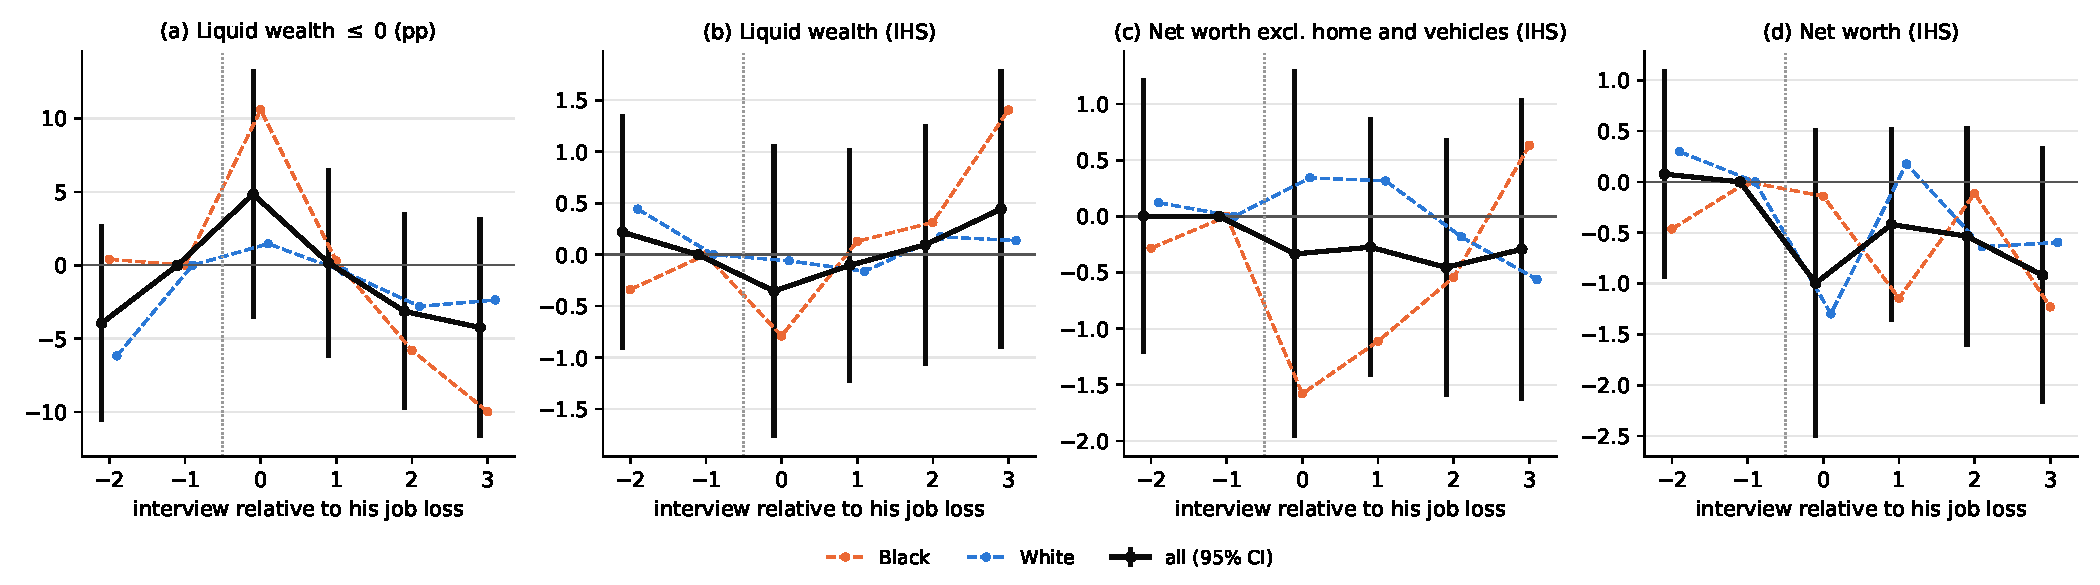
\includegraphics[width=\textwidth]{fig_psid_wealth_event.pdf}
\caption{Wealth around the husband's displacement (PSID wealth waves 1999--2019)}\label{fig:wealth_event}
\begin{minipage}{0.95\textwidth}\footnotesize Stacked event study of the husband's first displacement (closure,
layoff or firing) in 2000--2018, by wealth interview relative to the job-end year (reference: the last interview
before it; interview bins as in Figure~\ref{fig:consumption}), for husbands displaced alone (wife not displaced in the
three years around his job loss), against couples without a displacement; married couples with the wife aged 25--59;
father $\times$ stack and wave $\times$ stack fixed effects; 95\% confidence intervals for all couples clustered by
1968 family (473 displaced husbands, 51 of them with a joint loss estimated separately, 15{,}741 control stacks);
dashed lines: Black and White couples. (a) Liquid wealth (checking and savings, bonds, stocks, minus unsecured debt)
of zero or less, in points; (b)--(d) inverse hyperbolic sine of liquid wealth, of net worth excluding home equity and
vehicles, and of net worth, in 2000 dollars. Means over the first three interviews after the job loss: (a)
$-2.4$ (s.e.\ 3.0, $p=0.41$); (b) $0.15$ (0.53, $p=0.78$); (c) $-0.34$ (0.52, $p=0.51$); (d) $-0.62$ (0.48,
$p=0.19$). At the last interview before the loss, 59.5\% of the displaced husbands' families hold liquid wealth of
zero or less. Unsecured debt is netted in liquid wealth and not shown separately. Code:
\texttt{47.PSIDConsumptionEvent.py --wealth} with the definitions of \texttt{77.WealthDefinitions.py}
(\texttt{output/psid\_wealth\_event.csv}).\end{minipage}
\end{figure}
